\documentclass[../piano_di_qualifica.tex]{subfiles}
\begin{document}
\subsection{Primo periodo (RR)}
\label{sub:periodo-RR}
\subsubsection{Risultati controlli di qualità fase di analisi}
Qui di seguito verranno presentati i resoconti relativi ai test effettuati nella fase di analisi.

\begin{center}
	\begin{longtable}{|p{4cm}|p{4cm}|c|c|c|}
		\hline
		\rowcolor{lightgray}
		\textbf{Obiettivo}                    & \textbf{Metrica}              & \textbf{Risultato}        & \textbf{Accettabile} & \textbf{Esito} \\
		\hline
		\endfirsthead

		\hline
		\rowcolor{lightgray}
		\textbf{Obiettivo}                    & \textbf{Metrica}              & \textbf{Risultato}        & \textbf{Accettabile} & \textbf{Esito} \\
		\hline
		\endhead

		\hline
		\rowcolor{white}
		\multicolumn{5}{|c|}{\emph{Continua alla pagina successiva...}} \\
		\hline
		\endfoot
		\endlastfoot
		OPR01 Scadenze                        & MPR01 Varianza pianificazione & 14 giorni                 & $\leq$ 4             & Non Superato   \\
		OPR02 Budget parziale intaccato       & MPR02 Varianza costi parziali & $>$ 5\%                   & 0\%                  & Non Superato   \\
		OPR03 Budget finale intaccato         & MPR03 Varianza costi totali   & Budget totale intatto     & 0\%                  & Superato       \\
		OPR04 Versionamento                   & MPR04 Versionamento           & $>$25                     & $>$25                & Superato       \\
		OPR07 Rischi non previsti             & MPR07 Rischi inattesi         & $>$2                      & 2                    & Non Superato   \\
		OPR08 Rispetto obiettivi              & MPR08 Obiettivi soddisfatti   & 100\%                     & 100\%                & Superato       \\
		OPR09 Rispetto delle norme            & MPR09 Norme rispettate        & 100\%                     & 100\%                & Superato       \\
		OPR12 Verifica documenti              & MPR10 Frequenza controllo     & Ogni Milestone e modifica & Ogni Milestone       & Superato       \\
		OPD01 Leggibilità testo               & MPD01 Indice di Gulpease      & 73                        & \(\ge 60\)           & Superato       \\
		OPD02 Correttezza ortografica         & MPD02 Errori ortografici      & 0                         & 0                    & Superato       \\
		OPS03 Assenza file senza intestazione & MPS03 File senza intestazione & 0                         & 0                    & Superato       \\
		\hline
		\rowcolor{white}
		\caption{Esiti test fase di analisi}
	\end{longtable}
\end{center}

\subsubsection{Esiti verifica indici di Gulpease}
\label{sub:verif_gul_RR}

\begin{center}
	\begin{longtable}{|l|c|c|}
		\hline
		\rowcolor{lightgray}
		\textbf{Documento}                 & \textbf{Risultato} & \textbf{Esito} \\
		\hline
		\endfirsthead

		\hline
		\rowcolor{lightgray}
		\textbf{Documento}                 & \textbf{Risultato} & \textbf{Esito} \\
		\hline
		\endhead

		\hline
		\rowcolor{white}
		\multicolumn{3}{|c|}{\emph{Continua alla pagina successiva...}} \\
		\hline
		\endfoot
		\endlastfoot

		Analisi Dei Requisiti v1.0.0       & 72                 & Superato       \\
		Piano di Progetto v1.0.0           & 70                 & Superato       \\
		Piano di Qualifica v1.0.0          & 63                 & Superato       \\
		Norme di Progetto v1.0.0           & 71                 & Superato       \\
		Studio di Fattibilità v1.0.0       & 71                 & Superato       \\
		Glossario v1.0.0                   & 66                 & Superato       \\
		Verbale Interno 2020-11-25 v1.0.0  & 73                 & Superato       \\
		Verbale Interno 2020-12-10 v1.0.0  & 86                 & Superato       \\
		Verbale Interno 2020-12-21 v1.0.0  & 72                 & Superato       \\
		Verbale esterno 2020-12-17  v1.0.0 & 76                 & Superato       \\
		Verbale esterno 2021-01-08  v1.0.0 & 60                 & Superato       \\
		\hline
		\rowcolor{white}
		\caption{Esiti valutazioni dei documenti}
	\end{longtable}
\end{center}

\begin{figure}[H]
	\centering
	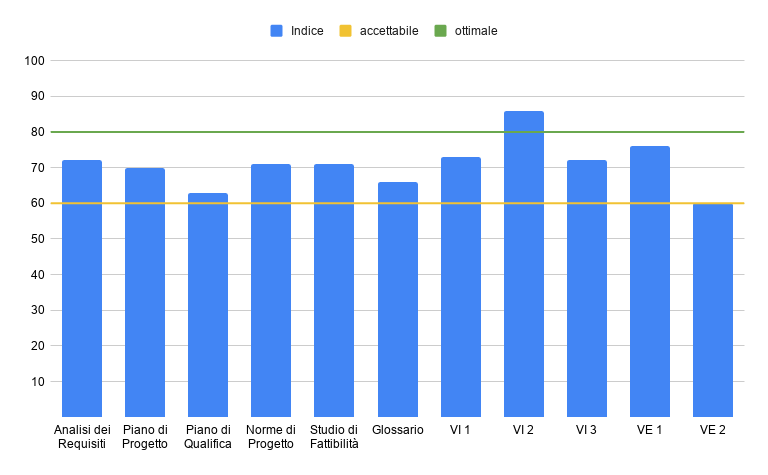
\includegraphics[width=14cm]{img/media_gul_RR.png}
	\caption{Andamento Indice di Gulpease}
\end{figure}

\subsubsection{Considerazioni sui risultati e sull’esito della revisione}
I risultati ottenuti dall’esito della revisione sono stati poco soddisfacenti a livello personale, mentre i colloqui e commenti si sono rivelati essenziali e esaustivi al fine di comprendere le modifiche da apportare e soprattutto realizzare un prodotto migliore. \\
Dopo l'esito ci siamo resi conto degli errori e delle imperfezioni fatte, e come poter ovviare a questi in modo da produrre un prodotto migliore, vedi \S\ref{par:retrospettiva-RR}. \\
Abbiamo inoltre compreso la necessità di pianificare meglio le nostre attività e soprattutto di considerare ulteriori rischi che si possono verificare nello svolgimento del progetto.


\subsection{Secondo periodo (RP)}
\label{sub:periodo-RP}
\subsubsection{Risultati test fase di progettazione e codifica della technology baseline}
Qui di seguito verranno presentati i resoconti relativi ai controlli di qualità effettuati nella fase di progettazione e codifica della technology baseline.

\begin{center}
	\begin{longtable}{|p{4cm}|p{4cm}|c|c|c|}
		\hline
		\rowcolor{lightgray}
		\textbf{Obiettivo}                    & \textbf{Metrica}              & \textbf{Risultato}        & \textbf{Accettabile} & \textbf{Esito} \\
		\hline
		\endfirsthead

		\hline
		\rowcolor{lightgray}
		\textbf{Obiettivo}                    & \textbf{Metrica}              & \textbf{Risultato}        & \textbf{Accettabile} & \textbf{Esito} \\
		\hline
		\endhead

		\hline
		\rowcolor{white}
		\multicolumn{5}{|c|}{\emph{Continua alla pagina successiva...}} \\
		\hline
		\endfoot
		\endlastfoot
		OPR01 Scadenze                          & MPR01 Varianza pianificazione & 0                         & $\leq$ 4             & Superato       \\
		OPR02 Budget parziale intaccato         & MPR02 Varianza costi parziali & $<$ 5\%                   & 0\%                  & Superato       \\
		OPR03 Budget finale intaccato           & MPR03 Varianza costi totali   & Budget totale intatto     & 0\%                  & Superato       \\
		OPR04 Versionamento                     & MPR04 Versionamento           & $>$25                     & $>$25                & Superato       \\
		OPR05 Adempimento requisiti obbligatori & MPR05 Requisiti obbligatori   & 100\%                     & 100\%                & Superato       \\
		OPR07 Rischi non previsti               & MPR07 Rischi inattesi         & 0                         & 2                    & Superato       \\
		OPR08 Rispetto obiettivi                & MPR08 Obiettivi soddisfatti   & 100\%                     & 100\%                & Superato       \\
		OPR09 Rispetto delle norme              & MPR09 Norme rispettate        & 100\%                     & 100\%                & Superato       \\
		OPR12 Verifica documenti                & MPR10 Frequenza controllo     & Ogni Milestone e modifica & Ogni Milestone       & Superato       \\
		OPD01 Leggibilità testo                 & MPD01 Indice di Gulpease      & 71                        & \(\ge 60\)           & Superato       \\
		OPD02 Correttezza ortografica           & MPD02 Errori ortografici      & 0                         & 0                    & Superato       \\
		OPS03 Assenza file senza intestazione   & MPS03 File senza intestazione & 0                         & 0                    & Superato       \\
		\hline
		\rowcolor{white}
	\caption{Esiti test fase di progettazione e codifica della technology baseline}
\end{longtable}
\end{center}

\subsubsection{Esiti verifica indici di Gulpease}
\label{sub:verif_gul_RP}

\begin{center}
	\begin{longtable}{|l|c|c|}
		\hline
		\rowcolor{lightgray}
		\textbf{Documento}                & \textbf{Risultato} & \textbf{Esito} \\
		\hline
		\endfirsthead

		\hline
		\rowcolor{lightgray}
		\textbf{Documento}                & \textbf{Risultato} & \textbf{Esito} \\
		\hline
		\endhead

		\hline
		\rowcolor{white}
		\multicolumn{3}{|c|}{\emph{Continua alla pagina successiva...}} \\
		\hline
		\endfoot
		\endlastfoot

		Analisi Dei Requisiti v1.3.0      & 72                 & Superato       \\
		Piano di Progetto v1.4.1          & 66                 & Superato       \\
		Piano di Qualifica v1.1.3         & 64                 & Superato       \\
		Norme di Progetto v2.3.0          & 64                 & Superato       \\
		Glossario v1.1.0                  & 65                 & Superato       \\
		Verbale Interno 2021-03-05 v1.0.0 & 86                 & Superato       \\
		Verbale Interno 2021-02-12 v1.0.0 & 62                 & Superato       \\
		Verbale Interno 2021-02-17 v1.0.0 & 90                 & Superato       \\
		Verbale esterno 2021-02-17 v1.0.0 & 72                 & Superato       \\
		\hline
		\rowcolor{white}
		\caption{Esiti valutazioni dei documenti}
	\end{longtable}
\end{center}

\begin{figure}[H]
	\centering
	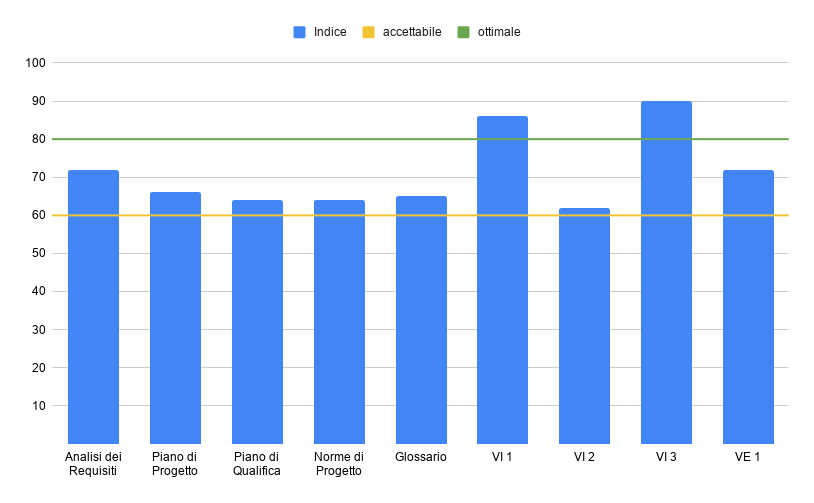
\includegraphics[width=14cm]{img/media_gul_RP.png}
	\caption{Andamento Indice di Gulpease in fase di progettazione e codifica della technology baseline}
\end{figure}

\subsubsection{Considerazioni sui risultati e sull’esito della revisione}
I risultati ottenuti dall'esito della revisione sono stati poco soddisfacenti perché hanno evidenziato la mancata comprensione delle precedenti segnalazioni. È stato necessario rivedere tutte le segnalazioni per comprenderle e poterle correggere. Ad esempio, nonostante l'incontro con il professore, il nuovo metodo di versionamento adottato si è rivelato essere sbagliato in quanto il gruppo ha mal interpretato i consigli ricevuti.
Questa seconda valutazione ha spronato l'approfondimento dei concetti di attività, rettificato la pianificazione grazie ad una comprensione corretta del modello incrementale e, più in generale, ha reso i membri del gruppo più critici verso i documenti prodotti.

\subsection{Terzo periodo (RQ)}
\label{sub:periodo-RQ}
\subsubsection{Risultati test fase di Revisione di Qualifica}
Qui di seguito verranno presentati i resoconti relativi ai controlli di qualità effettuati nella fase di Revisione di Qualifica.

\begin{center}
	\begin{longtable}{|p{4cm}|p{4cm}|c|c|c|}
		\hline
		\rowcolor{lightgray}
		\textbf{Obiettivo}                    & \textbf{Metrica}              & \textbf{Risultato}        & \textbf{Accettabile} & \textbf{Esito} \\
		\hline
		\endfirsthead

		\hline
		\rowcolor{lightgray}
		\textbf{Obiettivo}                    & \textbf{Metrica}              & \textbf{Risultato}        & \textbf{Accettabile} & \textbf{Esito} \\
		\hline
		\endhead

		\hline
		\rowcolor{white}
		\multicolumn{5}{|c|}{\emph{Continua alla pagina successiva...}} \\
		\hline
		\endfoot
		\endlastfoot
		TODO & TODO & TODO & TODO & TODO \\
		\hline
		\rowcolor{white}
	\caption{Esiti test fase di TODO}
\end{longtable}
\end{center}

\subsubsection{Esiti verifica indici di Gulpease}
\label{sub:verif_gul_RQ}

\begin{center}
	\begin{longtable}{|l|c|c|}
		\hline
		\rowcolor{lightgray}
		\textbf{Documento}                & \textbf{Risultato} & \textbf{Esito} \\
		\hline
		\endfirsthead

		\hline
		\rowcolor{lightgray}
		\textbf{Documento}                & \textbf{Risultato} & \textbf{Esito} \\
		\hline
		\endhead

		\hline
		\rowcolor{white}
		\multicolumn{3}{|c|}{\emph{Continua alla pagina successiva...}} \\
		\hline
		\endfoot
		\endlastfoot

		TODO & TODO & TODO \\
		\hline
		\rowcolor{white}
		\caption{Esiti valutazioni dei documenti}
	\end{longtable}
\end{center}

\begin{figure}[H]
	\centering
	%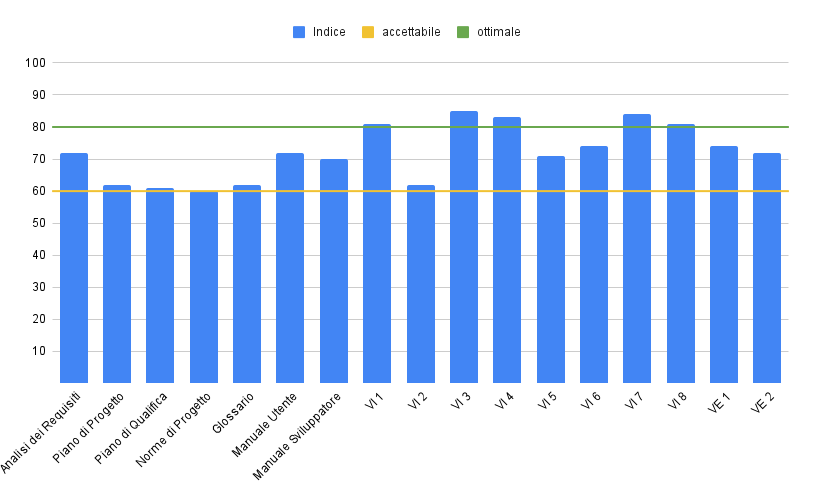
\includegraphics[width=14cm]{img/media_gul_RQ.jpg}
	\caption{Andamento Indice di Gulpease in fase di TODO}
\end{figure}

%\subsubsection{Considerazioni sui risultati e sull’esito della revisione}


\subsection{Riepilogo complessivo}
\label{sub:riepilogo_complessivo}

\subsubsection{Riepilogo test}
Nel seguente grafico, si può vedere un resoconto della quantità di test che sono stati superati o meno, divisi in base al periodo in cui sono stati fatti.

% TODO aggiornare con i dati della RQ
\begin{figure}[H]
	\centering
	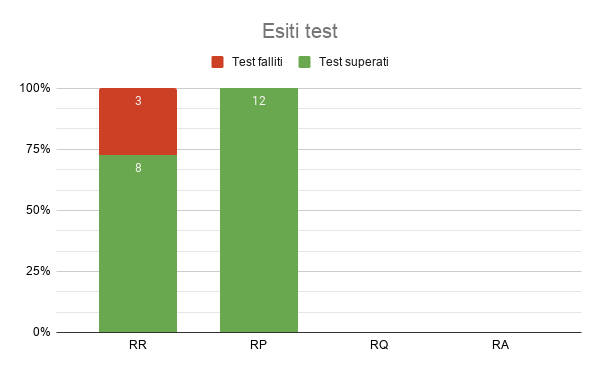
\includegraphics[width=14cm]{img/esiti_test.png}
	\caption{Test superati e falliti}
\end{figure}

\subsubsection{Riepilogo indici di Gulpease}
Nel seguente grafico, viene mostrata la media degli indici di Gulpease di tutti i documenti che sono stati consegnati divisi per periodo.

% TODO aggiornare con i dati della RQ
\begin{figure}[H]
	\centering
	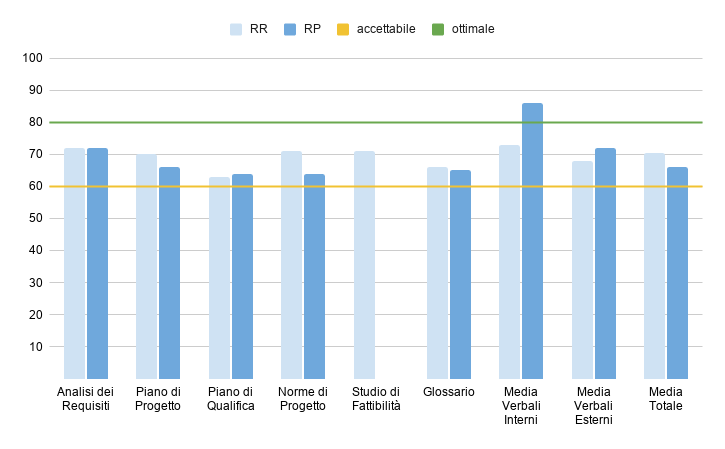
\includegraphics[width=14cm]{img/gulpease_documenti.png}
	\caption{Media indici di Gulpease}
\end{figure}

\end{document}
